\chapter{Theoretical Motivation} \label{chap-theory}


\section{The Standard Model of Particle Physics} \label{sec-StandardModel}

\begin{figure}
\begin{center}
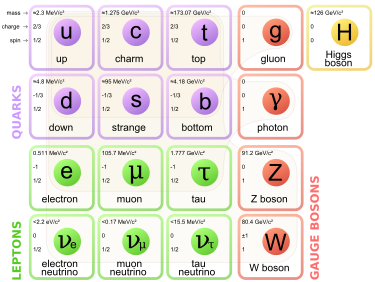
\includegraphics[width=0.9\textwidth]{Figures/StandardModel.png}
\end{center}
\caption{The Standard Model of particle physics.}
\label{fig-SM}
\end{figure}

The Standard Model (SM) of particle physics is the most successful physical theory to date, having been scrutinised and tested over and over 
again and still remaining strong. The SM is a quantum field theory that describes all known fundamental particles and their interactions with 
one another with the exception of gravity. It categorises fundamental particles and forces into three categories: three generations of quarks 
of type up and down, three generations of leptons, each linked to their corresponding neutrino type, and the forces. We can classify these 
categories into fermions, fundamental matter particles, and bosons, force particles carrying the quanta of the electromagnetic, weak, and 
strong forces. The three categories are shown in Figure \ref{fig-SM}. Each fundamental particle holds a property called ``spin'', which is the intrinsic angular momentum of that particle. Fermions are all spin-1/2 particles, whereas the bosons are all spin-1 particles --- with the exception of the Higgs, which has a spin of 0.

The Standard Model was first introduced in the 1960s when Sheldon Glashow first combined the weak and electromagnetic forces \cite{
Glashow:1961tr} to form an $SU(2)_L \otimes U(1)_Y$ gauge invariant electroweak model, which was then extended to incorporate the Higgs 
mechanism by Abdus Salam and Steven Weinberg \cite{PhysRevLett.19.1264, Salam:1959zz}. Quarks and gluons (the quanta of the strong force) were 
later found to posses a property called colour, whereby quarks are only able to exist as composite particle states called hadrons, with the 
exception of the top quark which has such a large mass that it does not undergo hadronisation. This property lead to the concept, and thus 
development, of quantum chromodynamics (QCD) \cite{GellMann:1964nj,PhysRevD.8.3633, PhysRevLett.30.1346}, described in more detail in Section 
\ref{subsec-QuantumChromodynamics}. The leptons differ from the quarks in that they interact only via the electromagnetic and weak 
interactions, where the neutrinos only interact via the weak force as they do not carry electric charge. This process is described in more 
depth in Section \ref{subsec-ElectroweakTheory}. These fundamental forces were combined in a gauge-invariant model, $SU(3)_C \otimes SU(2)_L \otimes U(1)_Y$,
to form the modern day for of the Standard Model. 

The masses of the fundamental particles are not explicitly stated in the Standard Model, it is with the introduction of the Higgs mechanism 
through the process of spontaneous symmetry breaking that they acquire mass with the introduction of the Yukawa terms (see Section \ref{subsec-ElectroweakSymmetryBreaking}).
It was thought that the neutrinos were considered massless until the recent discovery of oscillations between 
generations of neutrinos \cite{PhysRevLett.81.1562}, originally postulated by Bruno Pontecorvo in 1957 \cite{Pontecorvo:1967fh}. The first 
evidence for neutrino oscillations was published in 1998 in the study of atmospheric neutrinos in the Super-Kamiokande detector, Kamioka, 
Japan. 

The Higgs mechanism is the process responsible for the breaking of the electroweak symmetry in the gauge group $SU(2)_L \otimes U(1)_Y$, and 
thus the acquisition of mass in fundamental particles. Although first postulated in 1964 \cite{PhysRevLett.13.508, PhysRevLett.13.321, 
PhysRevLett.13.585}, the Higgs mechanism was only recently verified with the discovery of the Higgs boson with the ATLAS \cite{Aad:2012tfa} and 
CMS \cite{b846af59f42d440a9058d93ed5df44cf} experiments at the Large Hadron Collider (LHC), CERN. This Higgs mechanism essentially completes 
our picture of the Standard Model, with the exception of various short-comings described in Section \ref{subsec-SMFailures}.


\subsection{Gauge theory}

Almost all of the physics within Standard Model arises directly from imposed symmetries. Interactions are produced by requiring local gauge 
invariance under specific symmetry groups. We define the Standard Model in group theory as the unification of two gauge symmetry groups, 
describing the electroweak and strong interactions. The Glashow-Weinberg-Salam electroweak model sees the electromagnetic and weak interactions 
combined to create the electroweak gauge symmetry group $SU(2)_L \otimes U(1)_Y$, where the gauge symmetry group for strong interactions is 
defined as $SU(3)_C$. Thus, we can define the gauge symmetry group of the Standard Model to be 

\begin{equation}
SU(3)_C \otimes SU(2)_L \otimes U(1)_Y.
\end{equation}

In order to explain the concept of gauge invariance we start by considering changes to the phase of the wave-functions or fields. Let us take 
the Lagrangian density of a free Dirac field, $\psi$, describing all free-moving spin-$\frac{1}{2}$ fermions with a mass m:  

\begin{equation} \label{eqn-DiracLagrangian}
\lumi = \bar{\psi}(i \gamma^{\mu}\partial_{\mu}-m)\psi
\end{equation}

where $\gamma^{\mu}$ are the Dirac matrices. We can show that this is invariant under phase rotations, defined by

\begin{equation}
\psi \to \psi'= e^{i \theta}\psi, \quad \bar{\psi} \to \bar{\psi}' = e^{- i \theta}\bar{\psi},
\end{equation}

as the exponential factors will cancel each out, thus we have a $U(1)$ symmetry and corresponding conserved current. This is what is known as a 
global phase transformation due to the time dependency of $\theta$. However, we require a local gauge invariance, and therefore a local phase 
transformation must be applied such that $\theta$ is different at every space-time point, which we now define as $\theta (x_{\mu})$. The local 
phase transformations are applied to the wave function, $\psi$, and are defined in the following way:

\begin{equation}
\psi \to \psi'= e^{i \theta(x_{\mu})}\psi, \quad \bar{\psi} \to \bar{\psi}' = e^{- i \theta(x_{\mu})}\bar{\psi},
\end{equation} 

Dropping the space-time component $\mu$ from $x_{\mu}$ for simplicity, we can see that the Dirac equation is now not invariant under the local 
gauge transformation as

\begin{equation}
\partial_{\mu} (e^{i\theta(x)}\psi) = i(\partial_{\mu}\theta(x))e^{i\theta(x)}\psi + e^{i\theta(x)} \partial_{\mu}\psi 
\end{equation}

which we can then express in terms of the Lagrangian as

\begin{equation}
\lumi \to \lumi - [\partial_{\mu} \theta(x)] \bar{\psi} \gamma^{\mu} \psi.
\end{equation}

In order to restore local gauge invariance, we start by hypothesising that the fermions interact with a ``gauge field" $A_{\mu}$. We can then 
redefine our the interacting fermion Lagrangian 

\begin{equation} 
\lumi = \bar{\psi}(i \gamma^{\mu}D_{\mu}-m)\psi
\end{equation}

where we replace the ordinary derivative, $\partial_{\mu}$ covariant derivative, $D_{\mu}$, defined as

\begin{equation}
\partial_{\mu} \to D_{\mu} = \partial_{\mu} + iqA_{\mu}.
\end{equation}

where

\begin{equation}
A_{\mu} \to A_{\mu} - \partial_{\mu} \theta (x).
\end{equation}

In this way the gauge transformation of the fields cancel with that of the fermion fields, and therefore invariance is restored. The Lagrangian 
of Equation \ref{eqn-DiracLagrangian} is exactly what we expect for a fermion in an electromagnetic field with charge q. The second term that we obtain when we expand the 
Lagrangian, $-q\bar{\psi}\gamma^{\mu}A_{\mu}\psi$, describes the interaction of a fermion with a vector field with coupling strength $q=Qe$, 
where Q is the charge of the particle in units of e, where e is the electromagnetic coupling constant. By forcing a local $U(1)$ gauge 
invariance, we have essentially introduced quantum electrodynamics (QED), with the exception of the gauge field (photon) kinematic term 
described by the field strength tensor, $F_{\mu \nu}$, denoted  

\begin{equation}
F^{\mu \nu} = \partial^{\mu}A^{\nu} - \partial^{\nu}A^{\mu}
\end{equation}

and thus we obtain the gauge-invariant QED Lagrangian density:

\begin{equation}
\lumi_{QED} = \bar{\psi}(i \slashed{D}_{\mu} - m) \psi - \frac{1}{4}F_{\mu \nu}F^{\mu \nu}
\end{equation}

where $\slashed{D}_{\mu}$ is equal to $\gamma^{\mu}(\partial_{\mu} + iqA_{\mu})$.

We note that the gauge field $A_{\mu}$ is required to be massless in order to satisfy invariance under a local gauge transformation. This 
property arises as the gauge field mass term $m^2A_{\mu}A^{\mu}$ would explicitly break the gauge invariance, and thus must be removed from the 
Lagrangian density. Therefore we can say that QED describes Dirac fields, such as electrons and positrons, interacting with Maxwell 
electromagnetic force fields, photons.

By requiring local gauge invariance of the Lagrangian density by introducing additional fields in order to make it covariant with respect to an extended group of local transformations, we describe the gauge principle that is a fundamental process in particle physics. For the case of QED, we have a group of $1 \times 1$ unitary matrices multiplied by the Dirac field. The set of transformations form the Lie group $U(1)$, a group that is commutative, and thus Abelian. Gauge principle or local gauge invariant transformations can be applied to any $SU(N)$ group; Chen Ning Yang and Robert Mills first produced a theory of the $SU(2)$ gauge group \cite{PhysRev.96.191}, which was later extended to an $SU(3)$ gauge group to create QCD.  

\subsection{The Electroweak Theory} \label{subsec-ElectroweakTheory}

A theory for the unification of the electromagnetic and weak forces was first proposed by the American physicist Sheldon Glashow in 1961 \cite{Glashow:1961tr} and was later independently revised by Steven Weinberg in 1967 \cite{PhysRevLett.19.1264} and Abdus Salam \cite{Salam:1959zz} with the introduction of massive vector bosons acquiring mass by the process of spontaneous symmetry breaking. The GSW electroweak model later saw the authors receive the Nobel prize in physics in 1979. The GSW electroweak theory requires a unification of the gauge groups $SU(2)_L \otimes U(1)_Y$, where the definition of the $U(1)$ group from the previous section now refers to the unitary group of $1 \times 1$ matrices with respect to the weak hypercharge, Y, defined as 

\begin{equation}
Q = I_W + \frac{Y}{2}
\end{equation}

where Q is the electric charge, and $I_W$ is the weak isospin, also denoted $I_3$. The weak force is the only force known to violate parity, and thus distinguish between right- and left-handedness and confirmed in 1957 \cite{PhysRev.105.1413}. We can thus define left-handed doublets and right-handed singlets for fermions as so

\begin{equation}
\begin{pmatrix}
u_L \\
d_L
\end{pmatrix}
,u_R,d_R;
\quad
\begin{pmatrix}
c_L \\
s_L
\end{pmatrix}
,c_R, s_R;
\quad
\begin{pmatrix}
t_L \\
b_L
\end{pmatrix}
,t_R, b_R;
\end{equation}

for each generation of quark, and

\begin{equation}
\begin{pmatrix}
\nu_{e,L} \\
e_L
\end{pmatrix}
,e_R;
\quad
\begin{pmatrix}
\nu_{\mu,L} \\
\mu_L
\end{pmatrix}
,\mu_R;
\quad
\begin{pmatrix}
\nu_{\tau,L} \\
\tau_L
\end{pmatrix}
,\tau_R;
\end{equation}

for each generation of leptons. 

Left-handed quark and lepton doublets have weak isospin values of $I_W = 1/2$ where the upper and lower particle in each have $I^3_W = +1/2$ and $-1/2$, respectively. Right-handed particles are defined as singlets under the $SU(2)_L \otimes U(1)_L$ gauge group symmetry and thus have weak isospin of $I_W = 0$. We define left- and right-handedness by applying projection operators to the fields, such that

\begin{equation}
\psi = \frac{1}{2}(1-\gamma^5)\psi + \frac{1}{2}(1+\gamma^5)\psi = \psi_L + \psi_R,
\end{equation}

where we define the $\gamma^5$ matrix as the product of all the gamma matrices

\begin{equation}
\gamma^5 = i\gamma^0 \gamma^1 \gamma^2 \gamma^3 = 
\begin{pmatrix}
0 & 1 \\
1 & 0
\end{pmatrix}
\end{equation}

such that $\left(\gamma^5\right)^2$ is equal to the $4 \times 4$ identity matrix.

% Gell-Mann 1964 \cite{GellMann:1964nj}

Analogous to the previous case describing the $U(1)$ electromagnetic gauge group, the full covariant derivative for the electroweak theory within a $SU(2)_L \otimes U(1)_L$ gauge symmetry is given by

\begin{equation}
\partial_{\mu} \to D_{\mu} = \partial_{\mu} - ig I_W \textbf{T}^i\textbf{W}^i_{\mu} - i\frac{g'}{2}YB
\end{equation}

The $g$ and $g'$ terms represent the coupling constants for the $SU(2)_L$ and $U(1)_Y$ gauge groups, respectively; $\textbf{T}^i$ represents the three generators of the $SU(2)_L$ gauge group defined by the Pauli matrices 

\begin{equation}
\sigma_1 = 
\begin{pmatrix}
0 & 1 \\
1 & 0
\end{pmatrix}
,
\quad
\sigma_2 =
\begin{pmatrix}
0 & -i \\
i & 0
\end{pmatrix}
,
\quad 
\sigma_3 = 
\begin{pmatrix}
1 & 0 \\
0 & -1
\end{pmatrix}. 
\end{equation}

$W^i_{\mu}$ are the gauge fields that are now introduced conserve invariance in the gauge symmetry group $SU(2)_L$; and $B$ is the new gauge field for the conservation of invariance in the $U(1)_Y$ gauge symmetry group. For right-handed particle singlets, the generators $\textbf{T}^i$ are equal to 0, and thus the second term in the electroweak covariant derivative vanishes, there we can define the electroweak Lagrangian density as such

\begin{equation}
\begin{split}
\lumi_{EWK} & = \bar{\psi}_L \gamma^{\mu} \left(i \partial_{\mu} - g I_W \textbf{T}^i \cdot \textbf{W}_{\mu} - \frac{g'}{2} Y B_{\mu}\right)\psi_L \\
& + \bar{\psi}_R \gamma^{\mu}\left(i \partial_{\mu} - \frac{g'}{2} Y B_{\mu}\right)\psi_R - \frac{1}{4}\textbf{W}_{\mu \nu}\textbf{W}^{\mu \nu} - \frac{1}{4} B_{\mu \nu} B^{\mu \nu} .
\end{split}
\end{equation}

Here we define $\psi_L$ and $\psi_R$ as the double and singlet fields. Although we introduce the gauge fields $\textbf{W}^i_{\mu}$ and $ B_{\mu}$ to conserve invariance, they have no direct physical relation to gauge bosons. Instead we combine the gauge fields to form physical gauge bosons in the following linear combinations:

\begin{align}
W^{\pm}_{\mu} & = \frac{1}{\sqrt{2}}(W^1_{\mu} \pm iW^2_{\mu}), \\
Z_{\mu} & = -B_{\mu}\sin\theta_W + W^3_{\mu}\cos\theta_W, \\
A_{\mu} & = B_{\mu}\cos\theta_W + W^3_{\mu}\sin\theta_W
\end{align}   

We form the physical fields of the $W^{\pm}$ and $Z^0$ bosons, and the photon ($A_{\mu}$) by the mixing of the $W^i_{\mu}$ and $B{\mu}$ gauge fields with respect to the weak mixing angle, $\theta_W$, where we define the electric charge as:

\begin{equation}
e = g'\cos\theta_W = g \sin\theta_W.
\end{equation}

At this point we have a theory of electroweak interactions that does not incorporate electromagnetism explicitly and where the introduction of a mass term would explicitly break invariance of the $SU(2)$ and $U(1)$ symmetries, due to the way in which right- and left-handed fermions coupling differently. Therefore, all particles must be massless in this theory. We solve this problem via the process of spontaneous symmetry breaking in the Higgs mechanism, described in Section \ref{subsec-ElectroweakSymmetryBreaking}.  

\subsection{Quantum Chromodynamics} \label{subsec-QuantumChromodynamics}

Quantum Chromodynamics (QCD) is the theory of interactions between quarks and gluons confined within hadrons by what is known as the strong force --- so called because of it's strength compared to the weak force. The theory is based upon the gauge symmetry group $SU(3)_C$, where C represents colour, the QCD analogue of electrical charge. The $SU(3)_C$ gauge group is non-Abelian under the requirement of local gauge invariance. From experimental evidence we see that quarks carry a conserved charge, which we define as ``colour" with three degrees of freedom, such that a quark can be represented as a multiplet of fields in colour space. 

\begin{equation}
r = 
\begin{pmatrix}
r \\
b \\
g
\end{pmatrix}
\end{equation}

Upon imposing invariance under $SU(3)$ gauge symmetry, we derive the Lagrangian density for QCD to be

\begin{equation}
\lumi_{QCD} = \bar{q}\left(\gamma^{\mu}\partial_{\mu} - m \right) q + g_s \left( \bar{q}\gamma^{\mu}T_a q \right) G^a_{\mu} - \frac{1}{4}G^a_{\mu \nu}G^{\mu \nu}_a
\end{equation}

where $T_a$ represents the eight generators of the $SU(3)$ gauge group defined by the Gell-Mann lambda matrices, each $T_a$ is a $3 \times 3$ matrix in colour space which do not commute with each other and are completely anti-symmetric under the swapping of any pair of indices, and thus satisfy the lie algebra relation  

\begin{equation}
[T_a, T_b] = if_{abc}T_c.
\end{equation}

The lambda matrices represent eight massless gluon gauge fields, where $f^{abc}$ are the structure constants responsible for gluon self-interactions that arises in the field strength tensor shown in Equation \ref{eqn-QCDFieldStrengthTensor}. We note that the colour matrices and Dirac matrices do not interact as they act on different vector spaces. 

\begin{equation} \label{eqn-QCDFieldStrengthTensor}
G^a_{\mu \nu} = \partial_{\mu}G^a_{\nu} - \partial_{\nu}G^a_{\mu} + g_s f^{abc}G^b_{\mu}G^c_{\nu}
\end{equation}

As a product of self-interaction we observe two distinct properties of QCD in the form of colour confinement and asymptotic freedom. 

In a similar manner to photon exchange, the forces resulting from this type of interaction scales as $1/r^2$ at large distances, r, and thus the energy required to break up a quark-antiquark bound state is therefore finite. We have never observed quarks in isolation, but only in bound states of quark-antiquark pairs, or three-quark baryonic couplings.  

\begin{figure}
\begin{center}
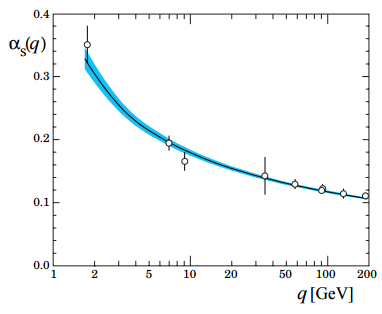
\includegraphics[width=0.5\textwidth]{Figures/AlphaS.png}
\end{center}
\caption{The experimentally measured values of the effective gauge coupling $\alpha_s(q)$ confirm the theoretically expected behaviour [Equation \ref{eqn-AlphaS}] at high energies (compilation of the Particle Data Group) \cite{AlphaS}}
\label{fig-AlphaS}
\end{figure}

Once we include higher-order corrections to our calculation we discover that the strength interactions mediated by vector bosons is dependent 
on the magnitude of q (energy-momentum transfer between partons), and it can be shown that the strong coupling constant, $\alpha_S$, can be 
defined as

\begin{equation} \label{eqn-AlphaS}
\alpha_s(q) = \frac{g_s(q)^2}{4\pi} = \frac{c}{log(q/\Lambda)} + ...
\end{equation}

where q is the energy-momentum transfer between partons, $\Lambda$ is the mass scale, and c is a constant. The logarithmic decay of the 
coupling is what we refer to as \textbf{asymptotic freedom} is observed in high-energy scattering (Figure \ref{fig-AlphaS}), such that the mass 
scale, $\Lambda$, has been determined to be $213^{38}_{-35}$ MeV \cite{Bethke:2000ai}\footnote{Here $\Lambda$ refers to a particular definition 
of the $\alpha_s$ called the $\overline{MS}$ scheme of dimensional regularisation.}. It is found that the strong coupling $\alpha_S$ decreases 
for interactions with higher energy, and is the reason that coloured particles are always found in colour-neutral states, as the coupling 
between the colour-charged states will be too strong and thus not be able to escape each other.

This prediction of QCD was first discovered in the early 1970s by H. David Polizer \cite{PhysRevLett.30.1346}, and by David J. Gross and Frank 
Wilczek \cite{PhysRevD.8.3633} in a completely independent study during the same year. They were subsequently awarded the Nobel prize in 
physics in 2004.

Another prominent aspect of QCD, which arises due to the increasing of the strong force as distance increases between quarks, is the property 
of \textbf{confinement}. As quarks continue to be pulled apart from one another, the energy rises sufficiently enough such that they 
form a colourless bound state, such as a quark-antiquark pair (meson), or three-quark baryonic state (baryon) as mentioned above. We call this 
process hadronisation, and is the reason we have never observed isolated quarks.  

%%%%%%%%%%%%%%%%%%%%%%%%%%%%%%%%%%%%%%%%%%%%%

\subsection{Electroweak Symmetry Breaking} \label{subsec-ElectroweakSymmetryBreaking}

The concept of spontaneous symmetry breaking of the electroweak symmetry first came to fruition in the 1960s and was postulated by the British 
physicist Peter Higgs \cite{PhysRevLett.13.508}, and independently by two groups: The first formed by the Belgian duo Francois Englert and 
Robert Brout \cite{PhysRevLett.13.321}, and the second by Gerald Guralnik, Carl Richard Hagen, and Tom Kibble \cite{PhysRevLett.13.585}.

we must spontaneously break the internal $SU(2)$ gauge symmetry by introducing an external field with a non-zero vacuum expectation value (vev),
$\phi_c(x)$. We therefore require an $SU(2)$ doublet of complex scalar fields, $\phi$, defined as

\begin{equation}
\Phi
= 
\begin{pmatrix}
\phi^+ \\
\phi^0
\end{pmatrix}
\end{equation}

The doublet of complex scalar fields has a weak isospin, $I_W = 1/2$, and hypercharge $Y = 1$ thus leading to $+1$ for the upper members of the doublet, and 0 for the lower. Thus, in terms of real scalar fields $\phi_i$, we set

\begin{equation}
\phi^+ = \frac{\phi_1 + i \phi_2}{\sqrt{2}}, \quad \phi^0 = \frac{\phi_3 + i\phi_4}{\sqrt{2}}.
\end{equation}

The Lagrangian density for the Higgs is then created by adding the scalar contribution to the massless GSW models

\begin{equation}
\lumi_{Higgs} = (D_{\mu}\phi)^{\dagger}(D^{\mu}\phi) - V(\phi)
\end{equation}

where $D_{\mu}$ is the electroweak covariant derivative defined in Section \ref{subsec-ElectroweakTheory} such that the conjugate $\phi^{\dagger}$encompasses the antiparticles $(\phi^-\bar{\phi^0})$, and $V(\phi)$ is input as the most general $SU(2)_L \otimes U(1)_Y$ invariant and renormalisable scalar potential defined as

\begin{equation}
V(\phi) = -\mu^2(\phi^{\dagger}\phi) + \lambda(\phi^{\dagger}\phi)^2.
\end{equation}

By defining $\lambda < 0$ and $\mu^2 < 0$ such that $\lumi_{Higgs}$ includes a wrong-sign mass term ($-\mu^2\phi^{\dagger}\phi$). This means that the potential that we defined is now bounded below such that there will be an invariant manifold of minima that lies below $V(\phi)=0$ as we wanted. This produces what is known as the ``mexican hat" potential, as can be visualised in Figure \ref{fig-MHP}.

\begin{figure} 
\begin{center}
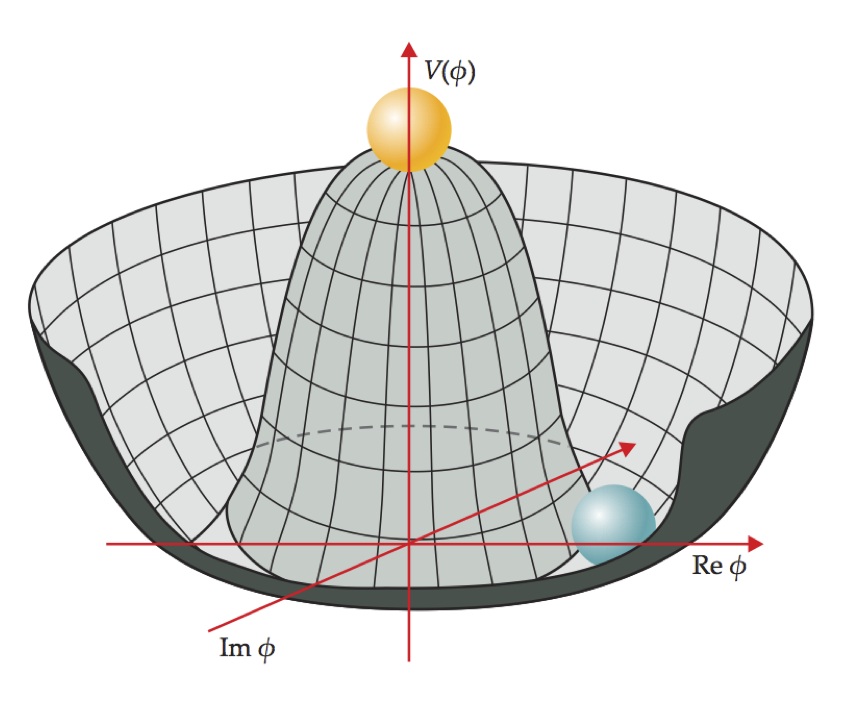
\includegraphics[width=0.7\textwidth]{Figures/MexicanHatPotential.png}
\end{center}
\caption{The ``Mexican Hat Potential" describing the vacuum expectation value of the Higgs in the real and imaginary planes, such that the minima lies below zero.}
\label{fig-MHP}
\end{figure}

We now see that $\lumi_{Higgs}$ is invariant under a local $SU(2)_L \otimes U(1)_Y$ gauge transformation 

\begin{equation}
\phi \to \phi' = exp[-ig\frac{T^i}{2}\cdot \Delta - i\frac{g'}{2}\Lambda]\phi.
\end{equation}

We define the minima of $V(\phi)$ to be 

\begin{equation}
\frac{dV}{d(\phi^\dagger\phi)} = 0 \rightarrow \mu^2 - 2\lambda(\phi^{\dagger}\phi) = 0
\end{equation}

such that the degenerate minima are

\begin{equation}
\phi^{\dagger}\phi|_{min} = \frac{\mu^2}{2\lambda} = \frac{v^2}{2}.
\end{equation}

We then want to spontaneously break the $SU(2)_L \otimes U(1)Y$ symmetry by choosing a minimum corresponding to the lowest energy state, or 
vacuum. The choice of vacuum direction is in fact arbitrary, however in order for the photon to remain massless we must assign a non-zero value 
to a neutral field, and thus we use the conventional notation

\begin{equation} \label{eqn-HiggsDoublet}
\braket{0|\phi|0} = \frac{1}{\sqrt{2}}
\begin{pmatrix}
0 \\
v
\end{pmatrix}.
\end{equation}

$\phi$ is then expanded around the selected minimum, where we set $\phi$ to $v + H$ where H is the neutral scalar Higgs field.

\begin{equation} \label{eqn-UnitaryGauge}
\phi = \frac{1}{\sqrt{2}}
\begin{pmatrix}
0 \\
v + H
\end{pmatrix}
\end{equation}

In this way the fields with vevs set to zero, also called the ``Goldstone" fields. We can see this by applying a local gauge transformation to 
the field. Thus we see that a gauge transformation of Equation \ref{eqn-UnitaryGauge} is a gauge transformation of $\phi$ with four independent 
scalar fields. From this we arises our three massless gauge bosons, the $W^{\pm}$ and $Z^0$ which gain mass and acquire three extra 
longitudinal polarisation degrees of freedrom by ``absorbing" the three unphysical Goldstone bosons. We can now write the Lagrangian density as 

\begin{equation} \label{eqn-HiggsLagrangian}
\begin{split}
\lumi_{Higgs} & = \frac{1}{2}(\partial_{\mu}H)(\partial^{\mu}H) + \frac{1}{4}g^2 (H^2 + 2vH + v^2) W^+_{\mu} W^{-\mu} \\
& + \frac{1}{8} (g^2 + g'^2) (H^2 + 2vH + v^2) Z_{\mu} Z^{\mu} \\
& - \mu^2 H^2 - \frac{\lambda}{4} (H^4 + 4vH^3)
\end{split}
\end{equation}

where we used to have the relation $(g\cos\theta_W + g'\sin\theta_W)^2 = g^2 + g'^2$, but now we can directly read off the masses of the $W^{\pm}$ and the $Z^0$ by extracting the mass terms $m^2_W W^+_{\mu}W^{-\mu}$ and $\frac{1}{2}M^2_Z Z_{\mu} Z^{\mu}$ from Equation \ref{eqn-HiggsLagrangian}, where the photon still remains massless as we would expect. We can then write the masses of the bosons as 

\begin{align}
M_W & = \frac{1}{2}gv \\
M_Z & = (g^2 + g'^2)^{\frac{1}{2}}v = \frac{1}{2} \frac{gv}{\cos\theta_W}.
\end{align}
 
For the Higgs scalar, we define the mass to be 

\begin{equation}
M_H = \sqrt{2}\mu = v\sqrt{2},
\end{equation}

and as a result of the above vector boson masses we note the following relation:

\begin{equation}
\frac{M_W}{M_Z} = \cos\theta_W.
\end{equation}

This vector boson mass relation is often called the ``weak $\Delta I = 1/2$" rule, and arises by our initial choice of Higgs doublet in order to perform spontaneous symmetry breaking.

We can then use the Higgs mechanism in a similar fashion to introduce the masses for all other fermions. We do so by introducing a gauge-invariant term in $SU(2)_L \otimes U(1)_Y$ which is responsible for interactions between the Higgs and fermion fields --- the Yukawa term. We can then write a generalised Standard Model Lagrangian with the additional Yukawa terms for the first generation of fermions as such: 

\begin{equation}
\lumi_{Yukawa} = -Y^{ij}_e \bar{l}^i_L \phi e^i_R - Y^{ij}_u \bar{q}^i_L \epsilon \phi^{\dagger} u^j_R - Y^{ij}_d \bar{q}^i_L \phi d^j_R + h.c.
\end{equation}

where the Yukawa couplings, $Y^{ij}_{e,u,d}$ (e,u,d = electron, up, down), are $3\times3$ complex matrices and $\epsilon$ is the $2\times2$ antisymmetric tensor. In the Standard Model fermion masses are generated through the coupling of the Yukawa couplings to the Higgs doublet (Equation \ref{eqn-HiggsDoublet}) such that we are obtain mass terms such as:

\begin{equation}
M_e = Y_e\frac{v}{\sqrt{2}}
\end{equation}

where here we have generated, in a gauge invariant system, a mass term for the electron. By construction, a resultant feature of the Yukawa couplings is that the couplings of the Higgs boson are proportional to the masses (or squares of the masses) of particles with which it interacts. This feature is integral to the phenomenology of Higgs searches. The discovery of the Higgs boson in 2012 by both the ATLAS \cite{Aad:2012tfa} and CMS \cite{b846af59f42d440a9058d93ed5df44cf} experiments with a mass of $\sim125$ GeV, and with couplings calculated to be consistent with the Standard Model \cite{Chatrchyan:2013lba, Aad:2013wqa}. proved to be another triumph for the Standard Model. So far, we have developed a picture where we do not encounter fermions of different generations. The most successful theory of quark interactions came in the form of the CKM matrix.

\subsection{The CKM matrix}

Inspired by early work from Murray Gell-Mann and Maurice L\'{e}vy, Italian physicist Nicola Cabibbo first introduced the Cabibbo rotation angle, $\theta_c$, in 1963 \cite{PhysRevLett.10.531} in order to preserve the universality of the weak interaction. The Cabibbo angle was built on the idea 
that there is a relative probability for a down-type quark to decay into an up-type quark. At that time only two generations of quark were 
known to exist, however the charm quark was still only theorised, and so the relative probabilities only described the mixing of the up, down,
and strange quark ($V_{ud}$ and $V_{us}$ ). It was also known that the probability of an up-type quark decaying to a down-type quark is zero, 
which is to say that quarks of the same up or down-type cannot mix without the help of a loop.

The angle, $\theta_c$, describes the rotation of the mass eigenstate vector space, formed by the mass eigenstates $\ket{d}$, $\ket{s}$, into the 
weak eigenstate vector space, formed by the weak eigenstates $\ket{d'}$ and $\ket{s'}$. From this we can say that the probability of an object 
coupling to an up-type quark through a charged weak interaction is a superposition of down-type quarks. This can be written as:

\begin{equation}
|d'> = V_{ud}\ket{d} + V_{us}\ket{s}
\end{equation}

or in terms of the Cabibbo angle 

\begin{equation}
|d'> = \cos\theta_c\ket{d} + \sin\theta_c\ket{s}
\end{equation}

Upon observing that CP violation could not be resolved within a four-quark model, Japanese physicists Makoto Kobayashi and Toshihide Maskawa 
sought to extend the Cabibbo rotation matrix to accommodate three generations of quark \cite{Kobayashi:1973fv}. This is written in the same 
manner as the Cabibbo rotation matrix, but including the top and bottom quark mixing phases, as seen in Equation \ref{eqn-ckm}, where d',s', 
and b' are the weak eigenstates written in terms of the mass eigenstates d,s,b. Kobayashi and Maskawa's predictions later came true when the 
bottom quark was discovered. Ever since the discovery of the bottom quark in 1977 at Fermilab, Chicago \cite{Innes:1977ae}, by a team led by 
Nobel prize-winning experimental physicist Leon Lederman, the top quark was theorised. The top quark was later discovered in 1995 with the CDF
\cite{PhysRevLett.74.2626} and D0 \cite{PhysRevLett.74.2422} experiments, also at Fermilab, and thus a full third generation of quarks was in 
place. Kobayashi and Maskawa subsequently won the Nobel prize in physics in 2008 for ``the discovery of the origin of the broken symmetry which 
predicts the existence of at least three families of quarks in nature".

\begin{equation} \label{equ-CKM}
\begin{pmatrix}
d' \\
s' \\
b' 
\end{pmatrix}
=
\begin{pmatrix}
V_{ud} & V_{us} & V_{ub} \\
V_{cd} & V_{cs} & V_{cb} \\
V_{td} & V_{ts} & V_{tb} 
\end{pmatrix}
\begin{pmatrix}
d \\
s \\
b 
\end{pmatrix}
\end{equation}

The CKM matrix describes the mixing of quark flavours where each term in the matrix represents the probability of that a quark transitioning 
into another quark. The values for each quark transition are given in Equation \ref{eqn-ckmValues} \cite{ckmValues}. We can see that the CKM matrix is essentially 
diagonal %%%%%%%%%%%%%%%%%%%%%%%%%%%%%

\begin{equation} \label{eqn-ckmValues}
V_{CKM}
=
\begin{pmatrix}
0.97427 \pm 0.00014 & 0.22536 \pm 0.00061 & 0.00355 \pm 0.00015 \\
0.22522 \pm 0.00061 & 0.97343 \pm 0.00015 & 0.0414 \pm 0.0012 \\
0.00886^{+0.00033}_{-0.00032} & 0.0405^{+0.0011}_{-0.0012} & 0.99914 \pm 0.00005
\end{pmatrix}
\end{equation}

\subsection{Where the Standard Model fails} \label{subsec-SMFailures}

The Standard Model of particle physics is has come under intense scrutiny for the past 50 years, and has always prevailed. Although the model is so finely crafted, it does not come without its failures. For example, as we know that neutrinos are in fact massive particles, we must incorporate new parameters to include the masses of the neutrinos. Despite all measurements conducted using all currently available experimental data describing the Standard Model to a high accuracy, there are still a number of questions that it does not answer:

\begin{itemize}
	\item What are the values of the neutrino mass parameters?
	\item Why is the top quark so much heavier than the other fundamental particles?
	\item Why is gravity not incorporated within the Standard Model?
	\item Can CP-violation explain the abundance of matter over anti-matter in the universe?
	\item Why is the electroweak scale so much smaller than the GUT scale and so much larger than the Planck scale? 
	\item What is Dark Matter and Dark Energy?
\end{itemize} 

At present we do not posses any definitive answers to any of these questions. However, there are a number of theoretical models motivated by Beyond the Standard Model (BSM) physics trying to address these problems. Unfortunately, we are yet to observe any evidence in agreement with any of these models. Some of the more prominent and accepted models to address problems in the Standard Model are listed below.

\begin{description}
	\item[Grand Unified Theory] A Grand Unified Theory (GUT) was one of the original ideas proposed to overcome problems in the SM. The premise is that the SM gauge group $SU(3)_C \otimes SU(2)_L \otimes U(1)_Y$ is actually just a subset of a larger gauge symmetry, the simplest of which is a $SU(5)$ gauge symmetry. This simplest case implies that $SU(5)$ has $5^2 - 1 = 24$ generators in the group, and thus 24 gauge bosons in the model, and thus 12 more gauge bosons than in the SM. In this new theory there are two stages of symmetry breaking, whereby the $SU(5)$ symmetry is broken at the GUT scale and the new bosons acquire mass, and at the electroweak scale symmetry breaking proceeds as usual. However, we can identify three problems with this theory: couplings do not unify at the GUT scale; why is the GUT scale higher than the electroweak scale; and protons are described to decay via the exchange of the new scalar bosons in the GUT model.
	\item[Hierarchy Problem] Most of the new physics models that are created are done so in order to overcome the so called \emph{hierarchy problem}, i.e. why is it that the electroweak scale is much larger than the Planck scale, where gravity is much stronger, and so much less than GUT scales? Usually when we refer to the hierarchy problem we refer to the technical hierarchy problem, relating to the mass of the Higgs boson. When considering the mass of the Higgs boson, we observe quantum corrections in the form of fermion loops, as shown in Figure \ref{fig-HiggsCorrections}. 
	\item[Technicolour] One of the oldest solutions to the hierarchy problem, Technicolour says that as the main problems arise from the inclusion of a fundamental scalar particle, they can be solved by not incorporating one. This is done by introducing a new set of gauge interactions, \emph{Technicolour}, which acts on the new ``technifermions". This process can be described in a similar manner to QCD with the use of different gauge groups. Technifermions are created in bound states with the lightest being the technipions, and using the Higgs mechanism, the longitudinal components of the $W^{\pm}$ and $Z^0$ bosons arise, generating the gauge boson masses. However, there must also be a mechanism whereby the technifermions acquire their masses. \emph{Extended Technicolour} models have been hard to construct which have not already been ruled out. This idea lost favour until recent models containing a ``little Higgs" have sparked a resurgence of the idea \cite{}.
	\item[Supersymmetry] In Supersymmetry (SUSY) we have for every fermionic degree of freedom a corresponding bosonic degree of freedom and visa versa. That is to say that each fermionic particle in the SM has two corresponding bosonic supersymmetric particles, with spin-0 for bosonic partners, and each bosonic SM particle has one fermionic supersymmetric particle with a spin of 1/2. The supersymmetric partners to SM particles can be seen, for the first generation at least, in Table \ref{tab-SUSYParticles}. In SUSY we require two Higgs doublets to give mass to both up- and down-type quarks such that the transformation is still invariant under a local gauge transformation. If we introduce a scalar loop into the Higgs propagator, as shown in Figure \ref{fig-SUSYHiggs}, we introduce a new contribution to the Higgs mass. This property is one of the main aspects of SUSY as introducing two scalars, with the same mass, for every fermion then cancels out the quadratic divergences. SUSY also incorporates dark matter by introducing a particle called the ``lightest supersymmetric particle" which is a dark matter particle candidate. 
	\item[Extra Dimensions] Another way to overcome the hierarchy principle comes in the form of extra dimensions. There are many models that describe the universe in more than 4 dimensions --- the most popular theories describe the universe in 10 or 11 dimensions. In these theories gravity is said to propagate through our current three dimensions into smaller extra dimensions, and thus leads to a reduction in the hierarchy between the electroweak and Planck scales.
\end{description}

\begin{figure}
\begin{center}
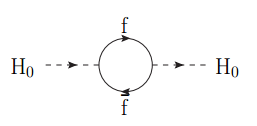
\includegraphics[width=0.4\textwidth]{Figures/HiggsCorrection.png}
\end{center}
\caption{Quantum correction to the mass of the Higgs boson via a fermion loop.}
\label{fig-HiggsCorrections}
\end{figure}

\begin{table}
\begin{center}
\begin{tabular}{cccc}
\hline
\hline
\textbf{SM Particle} & \textbf{Spin} & \textbf{SUSY Particle} & \textbf{Spin} \\
\hline
Electron & 1/2 & Selectron & 0 \\
Neutrino & 1/2 & Sneutrino & 0 \\
Up & 1/2 & Sup & 0 \\
Down & 1/2 & Sdown & 0 \\
\hline
Gluon & 1 & Gluino & 1/2 \\
\hline 
Photon & 1 & Photino & 1/2 \\
$Z^0$ & 1 & Zino & 1/2 Neutralinos \\
Higgs & 0 & Higgsino & 1/2 \\
\hline
$W^{\pm}$ & 1 & Wino & 1/2 Charginos \\
$H^+$ & 0 & Higgsino & 1/2 \\
\hline
\hline
\end{tabular}
\end{center}
\caption{Standard Model particles and their supersymmetric counterparts and spin values.}
\label{tab-SUSYParticles}
\end{table}

\begin{figure}
\begin{center}
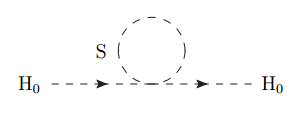
\includegraphics[width=0.4\textwidth]{Figures/SUSYHiggs.png}
\end{center}
\caption{The introduction of a new scalar boson loop in the Higgs boson propagator.}
\label{fig-SUSYHiggs}
\end{figure}

There are a number of ways of searching for BSM effects, including the following:

\begin{description}
	\item[Collider Experiments] If the theory is correct, then BSM particles should be detectable at collider experiments, such as the LHC, and decay to SM particles. These types of particles would be detected by all-purpose discovery machines like the ATLAS and CMS experiments.
	\item[Precision Experiments] By measuring SM processes to an extremely high precision, we are able to compare the results to theoretical prediction and measure any deviations. Experiments such as LEP ($e^+e^-$ collider) provide high precision measurements of the $Z^0$ pole, and the $g - 2$ experiment which measures the anomalous magnetic moment of the muon.
	\item[Rare Decay/Process Measurements] Measurements can be conducted my calculating the cross-section or decay rate of a rare decay/process which is predicted to be extremely small within the SM. Examples of such experiments include: the NA62 experiment, which measures rare decays of kaons, neutron electric dipole moment experiments, proton decay experiments, neutrino mixing experiments (T2K/SuperKamiokande), and CP violation experiments such as LHCb and Belle. 
\end{description}

In practice we see that several detection techniques are in fact complimentary to one another, for example CP-violation is a process that must be studied by dedicated experiments, however if the results from these experiments differ from that of the SM then there should be new particles which should be observable in collider experiments. 

\section{The Top Quark} \label{sec-TheTopQuark}

The top quark is the heaviest of all the fundamental particles and was first postulated, along with the bottom quark, in 1973 by Makoto 
Kobayashi and Toshihide Maskawa \cite{Kobayashi:1973fv} to explain the observations of CP violation in the kaon sector. It was with the 
discovery of the $\tau$ lepton \cite{PhysRevLett.35.1489} in 1975, and then the discovery of the bottom quark in 1977 \cite{Innes:1977ae} and 
the quark-lepton generation symmetry which lead to the postulation of the top quark. Event with the discovery of the W and Z bosons in 1985 
with the UA1 \cite{ARNISON1983103} and UA2 \cite{Banner1983476} experiments at the Super Proton Synchrotron (SPS), CERN, the top quark was 
still nowhere to be seen, and at this point in time there was still no experimental apparatus capable of reaching the required energies needed 
to discover the top. It was in 1995 when the CDF \cite{PhysRevLett.74.2626} and D0 \cite{PhysRevLett.74.2422} experiments at the Tevatron (
Fermilab, Illinois) first observed the top quark, which subsequently prompted Kobayashi and Maskawa to win the Nobel prize for their 
predictions in 2008.

The mass of the top quark is of critical importance due to the fact that the Yukawa coupling (coupling to the Higgs) of the top is close to 
unity, and is thus at the scale of electroweak symmetry breaking. Although the top quark mass is a vital parameter in the SM, there is a 
conceptual problem when defining the mass of the top. The problem arises when we consider free particles, such as leptons, where the mass is 
well defined, but when we consider confined states then there is no straight forward way in which we can measure the mass of that particle. We must infer the mass of the top and define a scheme by which to measure this property, noting that the value is subject to change depending on the scheme used. The two main interpretations of the top mass are the pole mass and minimal subtraction ($\overline{MS}$) schemes. When we consider the pole mass we treat the top mass as a physical mass term in the quark propagator, similar to any other free particle. This works well in perturbation theory, however the non-perturbative infra-red effects in QCD, additional loops from self-interacting gluons, are not accounted for in this scheme. In order to define a realistic and finite value for the mass of the top, a renormalisation scheme is introduced --- the $\overline{MS}$ scheme. The scheme is often called the running mass, due to its dependence on the renormalisation scale, $\mu$, which is essentially arbitrary. It is possible for the mass derived from the $\overline{MS}$ scheme to be calculated from the pole mass \cite{Melnikov:2000qh}, however the $\overline{MS}$ top quark mass can be extracted straight from data, and is thus a more preferential method. A recent result shows that, when incorporating electroweak corrections for a Higgs mass of 125 GeV, the difference between the pole and $\overline{MS}$ schemes results in around a 1 GeV difference \cite{Jegerlehner:2012kn}. 

The mass of the W boson and the top are two of the most important parameters to global electroweak fits constraining the Higgs potential. The most up-to-date measurement of the top mass has been calculated by combining results from the LHC and the Tevatron to be $m_{top} = 173.34 \pm 0.27(stat.) \pm 0.71(syst.)$ GeV/c$^2$ \cite{ATLAS:2014wva}. As a direct result of the top quarks extremely large mass, it has a very short decay time which is shorter than the time required for quarks to hadronise and form composite particles with other quarks. The decay time of the top is approximately $5 \times 10^{-25}$ s \cite{Quadt:2007jk}, whereas the hadronisation time for quarks is given as $\tau_{had.} \approx 1/\Lambda_{QCD} \approx 10^{-23}$ s \cite{0954-3899-37-7A-075021}. Thus, we never observe $t\bar{t}$ bound states and the information relating to spin is inherited by the decay products of the top. Therefore the top quark provides unique opportunities to study precision tests of the Standard Model.


\subsection{Top quark production at hadron colliders} \label{subsec-TopProduction}

There are two processes whereby top quarks are produced at hadron colliders: single top quark production via the electroweak interaction in 
association with a quark or a vector boson, and top quark pair ($t\bar{t}$) production where a top quark is produced with it's antiparticle 
through the strong interaction. The latter of the two is the most prevalent of the production sources, and thus provides the signature for this 
analysis. The leading order (LO) Feynman diagrams for the production of top quark pair and single top processes can be seen in Figures \ref{fig-ttbarProductionLHC} and \ref{fig-singletopProductionLHC}. Single top production is of particular significance as it allows direct measurement 
of the $Wtb$ vertex, and thus we are able to measure the magnitude of the CKM matrix element $|V_{tb}|$.

Due to the high centre-of-mass energy of the LHC, top quarks are produced in copious amounts such that it has obtained the title of ``top 
factory". Unlike the Tevatron, which did not have a high enough centre-of-mass energy to probe the properties of the top, the LHC is able to 
measure its properties to a high accuracy. The main production mechanism at the Tevatron saw quark-antiquark annihilation in 90\% \cite{
Kidonakis:2012db} of collisions due to the collision of protons and anti-protons, where the secondary production process was gluon-gluon fusion 
in 10\% of collisions. At the LHC the converse is true, such that gluon-gluon fusion is the most prominent process and top pairs are produced 
in this way 80\% of the time at $\sqrt{s} = 8$ TeV. The rate for top production through gluon-gluon fusion increases with energy, and will rise 
to around 90\% at $\sqrt{s} = 14$ TeV. The reason for this lies in the parton distribution functions (pdfs) and how the energy of a hadron is 
distributed with the increase of energy. As the energy increases the gluons carry a much larger fraction of the hadron's energy. At the 
Tevatron quark-antiquark annihilation can arise from valence quarks of the hadron, whereas at the LHC the quarks must originate from the ``sea" 
quarks. The increase in $t\bar{t}$ events produced by gluon-gluon fusion events implies that the probability of the production of initial state 
radiation is reduced, and thus the sensitivity to the $t\gamma$ vertex is increased.

One of the main observables in particle physics experiments is the production cross-section, $\sigma$, of a process. We define the cross-section for $\sigma_{i\to f}$ to be the probability for an initial statie, i, to transition into a final state, f. We calculate the cross-section of a process by convoluting the PDFs $f_1(x_i, \mu_F)$ and $f_2(x_j, \mu_F)$ of the initial particles (protons in this case) with the cross-section of the hard interaction process, $\hat{\sigma}_{i,j} \to t\bar{t}$, for all parton species $i,j$. We can also calculate the cross-section of top quark pairs with an associated particle, as measured in this analysis, as shown in Equation \ref{eqn-ttbarplusXcross-sect} below.

\begin{equation} \label{eqn-ttbarplusXcross-sect}
\sigma_{pp \to t\bar{t}+X} = \sum_{i,j} \int^1_0 dx_1 \int^1_0 dx_2 f_1(x_i, \mu_F)f_2(x_j, \mu_F)\hat{\sigma}_{i,j \to t\bar{t}}(\hat{s})
\end{equation}

\begin{figure} 
\begin{center}
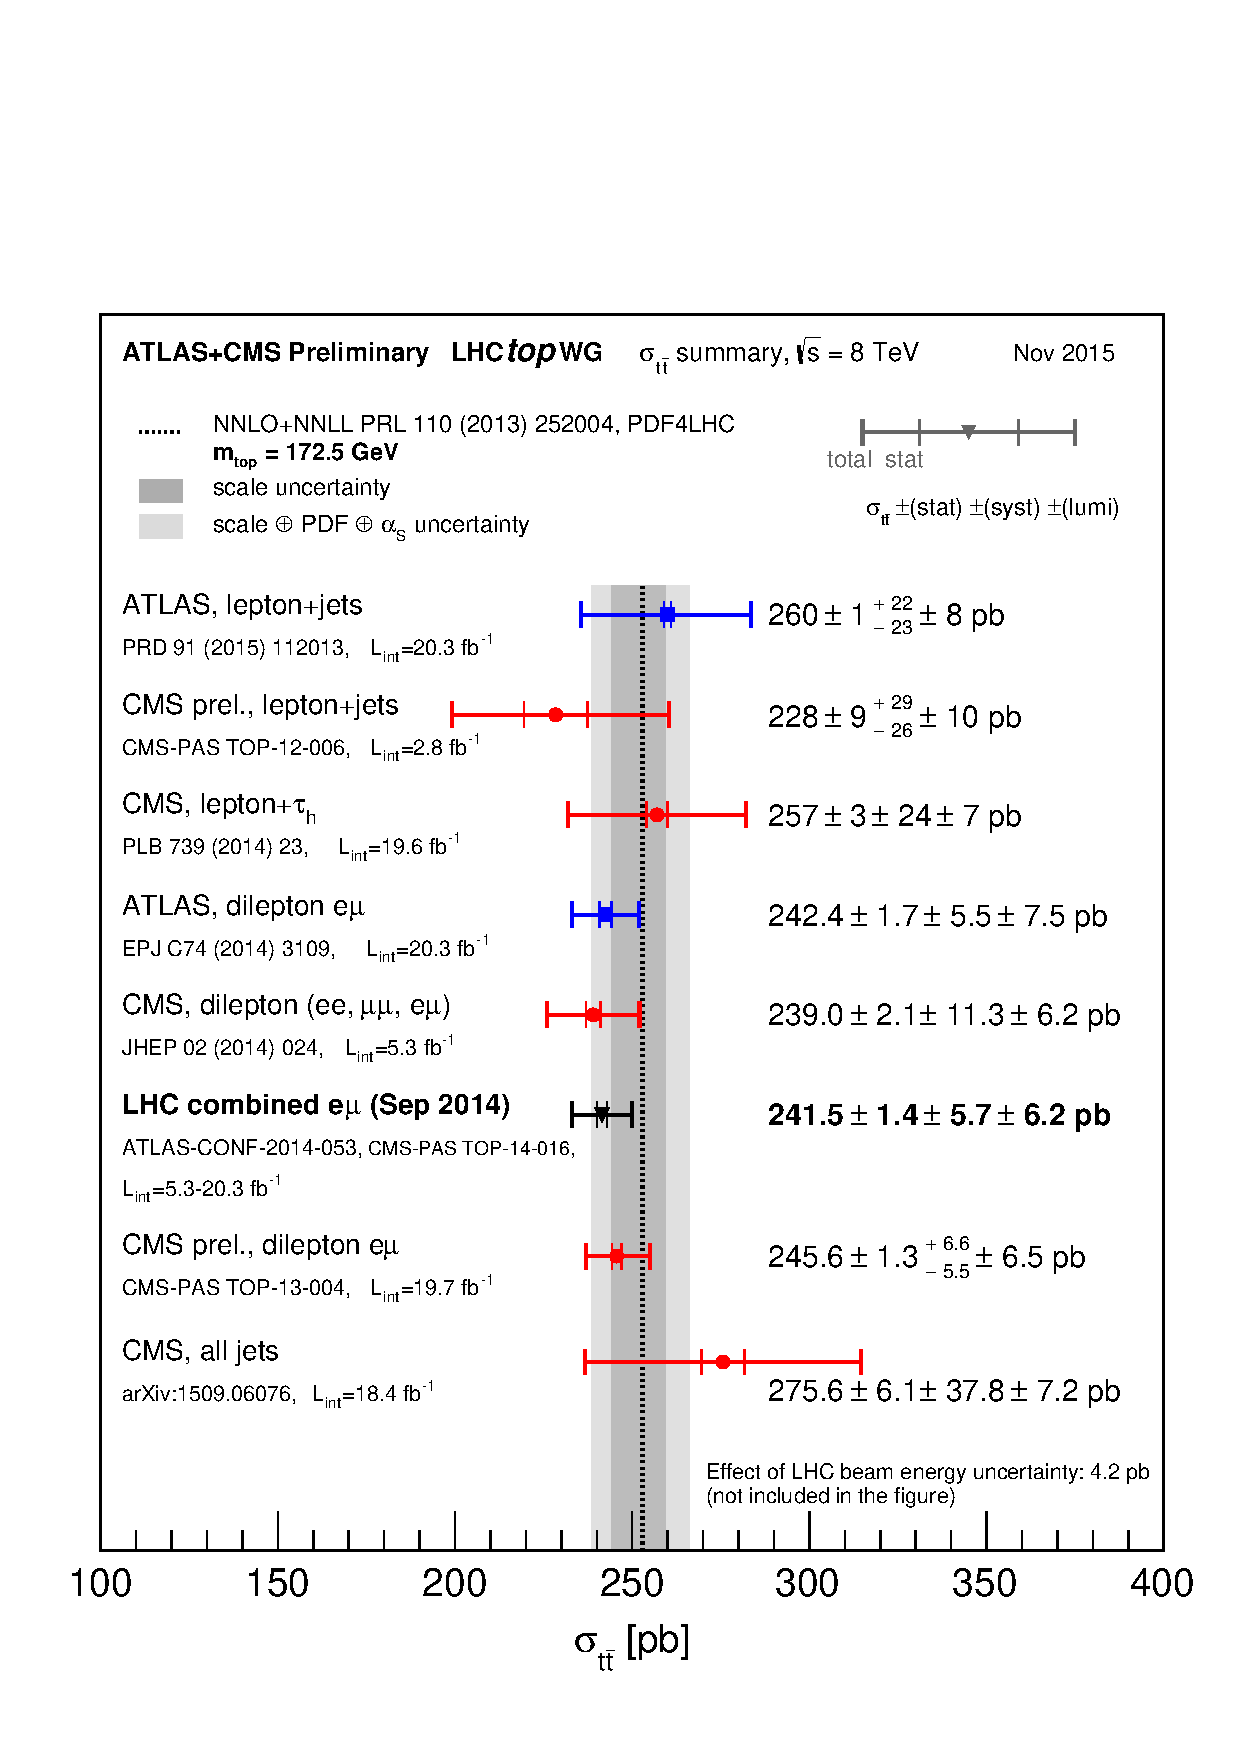
\includegraphics[width=0.8\textwidth]{Figures/ttbarCombinedXsect.pdf}
\end{center}
\caption{Summary of measurements of the top-pair production cross-section at 8 TeV compared to the exact NNLO QCD calculation complemented with NNLL re-summation (top++2.0). The theory band represents uncertainties due to renormalisation and factorisation scale, parton density functions and the strong coupling. The measurements and the theory calculation are quoted at $m_{top}=172.5$ GeV. \cite{ttbarXsectCombination}}
\label{fig-ttbarCombinedXsect}
\end{figure}

The production cross-section of top quark pair events has been measured by both the ATLAS and CMS experiments to be  \cite{} and \cite{}. The LHC $t\bar{t}$ cross-section can been in Figure \ref{fig-ttbarCombinedXsect}. We can see the value of the $t\bar{t}$ and single top production cross-sections for different centre-of-mass energies, as measured by the LHC and the Tevatron, in Table \ref{tab-ttbarcrosssections}. We see that as energy increases, the top quair pair production cross section increases. This is shown in Figure \ref{fig-ttbarXsectPlot}.

\begin{figure}
\begin{center}
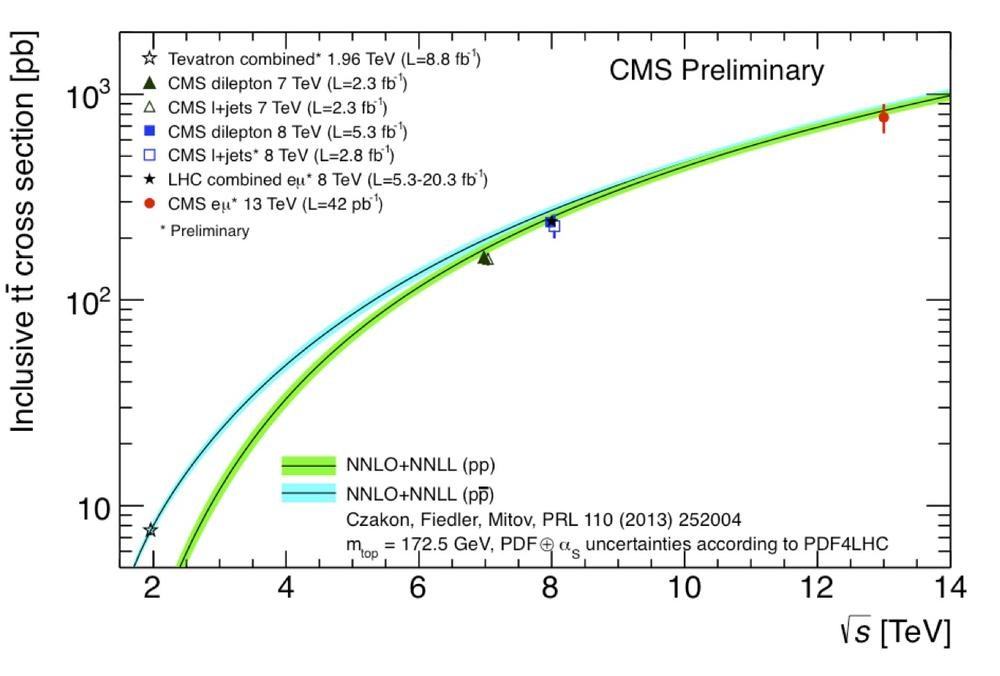
\includegraphics[width=0.7\textwidth]{Figures/ttbarXsectPlot.png}
\end{center}
\caption{Top quark pair production cross section measurements compared to the Standard Model predictions as a function of the center-of-mass energy. The new result of the CMS collaboration at 13 TeV is displayed in red and is in agreement with the theory prediction (green band). \cite{ttbarXsectPlot}}
\label{fig-ttbarXsectPlot}
\end{figure}

\begin{table}
\begin{center}
\begin{tabular}{lccccc}
\hline
\hline
& \textbf{$\sqrt{s}$} & \textbf{s-channel} & \textbf{t-channel} & \textbf{tW-channel} & \textbf{$t\bar{t}$} \\
\hline
Tevatron & 1.9 & 1.046 & 2.08 & 0.266 & 7.31 \\
LHC & 7 & 4.56 & 65.9 & 15.6 & 163 \\ 
 & 8 & 5.55 & 87.2 & 22.2 & 235.8 \\
 & 14 & 11.86 & 248 & 83.6 & 920 \\
\hline
\hline
\end{tabular}
\end{center}
\caption{The Standard Model cross-sections for both single top and $t\bar{t}$ processes at the Tevatron and the LHC. All cross-sections are calculated at next-to-next-to-leading-order and measured in pb. \cite{Czakon:2013goa}}
\label{tab-ttbarcrosssections}
\end{table}

\begin{figure} 
\begin{center}
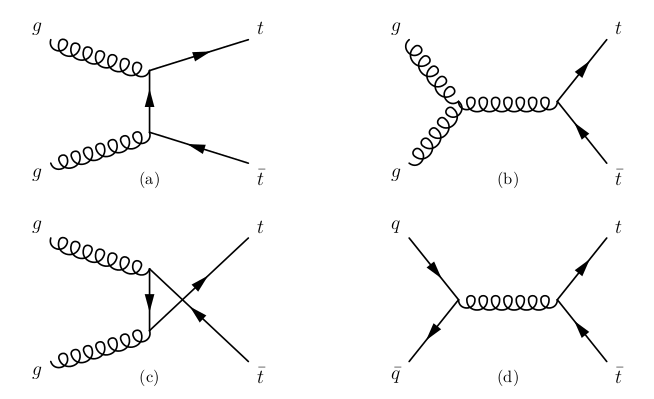
\includegraphics[width=0.9\textwidth]{Figures/ttbarProductionLHC.png}
\end{center}
\caption{Lowest level diagrams for $t\bar{t}$ production at the LHC. Gluon scattering processes, {(a)}, {(b)}, and {(c)}, are the dominant processes at LHC energies, while quark scattering, process {(d)}, is the dominant one at TeVatron energies. \cite{SergeyThesis}}
\label{fig-ttbarProductionLHC}
\end{figure}

\begin{figure} 
\begin{center}
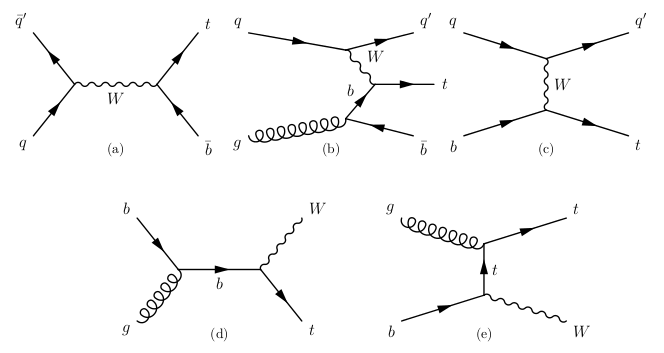
\includegraphics[width=\textwidth]{Figures/singletopProductionLHC.png}
\end{center}
\caption{Leading-order level diagrams for single top production at the LHC. {(a)} s-channel, {(b)} and {(c)} represent the t-channel, {(d)} and {(e)} both represent the two tW channels. \cite{SergeyThesis}}
\label{fig-singletopProductionLHC}
\end{figure}

\subsection{Top quark decay modes} \label{subsec-TopDecayModes}

We observe that the top quark decays to a W boson and a bottom quark ($t \to Wb$) almost 100\% of the time, as other decay modes to lighter quarks $t \to Wq$ (q=d,s) are highly Cabibbo suppressed by the Standard Model. This can be seen by examining the matrix elements of the CKM matrix for top decays, such that the value of $|V_{tb}|$ gives

\begin{equation}
|V_{tb}| = 0.999146^{+0.000021}_{-0.000046}
\end{equation}

from the unitarity requirement of the CKM matrix \cite{PhysRevD.86.010001}. The value of $|V_{tb}|$ can be measured by calculating the production cross-section of single top production, and the latest measurement is given to be \cite{Khachatryan:2014iya}:

\begin{equation}
|V_{tb}| = 0.998 \pm 0.038 (experimental) \pm 0.016 (theoretical)
\end{equation}

which lies in accordance with the unitarity condition imposed on the CKM matrix. 

Providing that the top decays to a W boson and b quark 100\% of the time, we then categorise into three distinct decay modes: fully leptonic, semi-leptonic, and fully hadronic. The three decay modes have branching fractions of 10.5\%, 43.8\%, and 45.7\%, respectively \cite{PhysRevD.86.010001}. The different channels can be visualised in Figure \ref{fig-ttbarDecay}.

\begin{description}
	\item[Fully leptonic] (Also called the di-leptonic or dilepton decay mode) denotes the decay mode of a top quark pair whereby both W legs decay to a lepton and a neutrino, with the exception of $\tau$ leptons. There is therefore three channels to observe with oppositely charged leptons in the final state: the di-muon, di-electron, and mixed electron and muon channels. Therefore we require dilepton events to have two leptons, and two b-tagged jets in the final state. The three decay channels have branching fractions of $1/81$ for same-flavour channels, and $2/81$ for mixed flavour final state modes. This mode provides the cleanest signature of the three decay modes within a hadronic environment, and thus a powerful tool for the measurement of top quark properties. The difficulty lies in the fact that there are two neutrinos in the final state, and thus a fourfold ambiguity in the full kinematic reconstruction.
	\item[Semi-leptonic] The semi-leptonic channel requires on of the W bosons to decay to a lepton and neutrino pair, and the other to two quarks, which subsequently hadronise to form two jets. This results in an event topology where we have one lepton, one neutrino, and 4 jets in the final state. This mode provides a easily accessible signature in the final state for electrons and muons, and has the advantage of having a larger branching fraction, with respect to the dilepton channel, and thus more events. Each semi-leptonic mode has a branching fraction of $12/81$.
	\item[Fully hadronic] In this case both of the W boson decay hadronically, and thus we have only jets in our final state. We do not consider this channel as the contamination from the QCD multijet background and the jet energy uncertainty is too large to carry out precision measurements. 
\end{description}

In this analysis we only consider the fully leptonic (or di-leptonic or dilepton) channel with the exclusion of $\tau$ leptons in the final state, as a $\tau$ lepton must be identified by its decay products, and adds extra uncertainty into the measurement. This channel has the quality that it provides a very clean signature in the detector, at least for a final state containing muons, as CMS excels at triggering and measuring muons. CMS also boasts a very high resolution electromagnetic calorimeter and thus it is ideal for measuring electrons and photons. This analysis focuses on the dilepton channel but with an associated photon radiated from any of the charged particles, as shown in Figure \ref{fig-ttgammaFeynmanDiagram}

\begin{figure} [h!]
\begin{center}
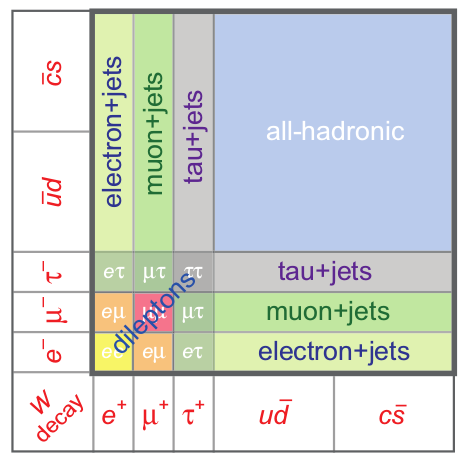
\includegraphics[width=0.5\textwidth]{Figures/ttbarDecayFractions.png}
\end{center}
\caption{Branching fractions of the W decays within top quark pairs. \cite{ttbarDecayFractions}}
\label{fig-ttbarDecay}
\end{figure}

\begin{figure} 
\begin{center}
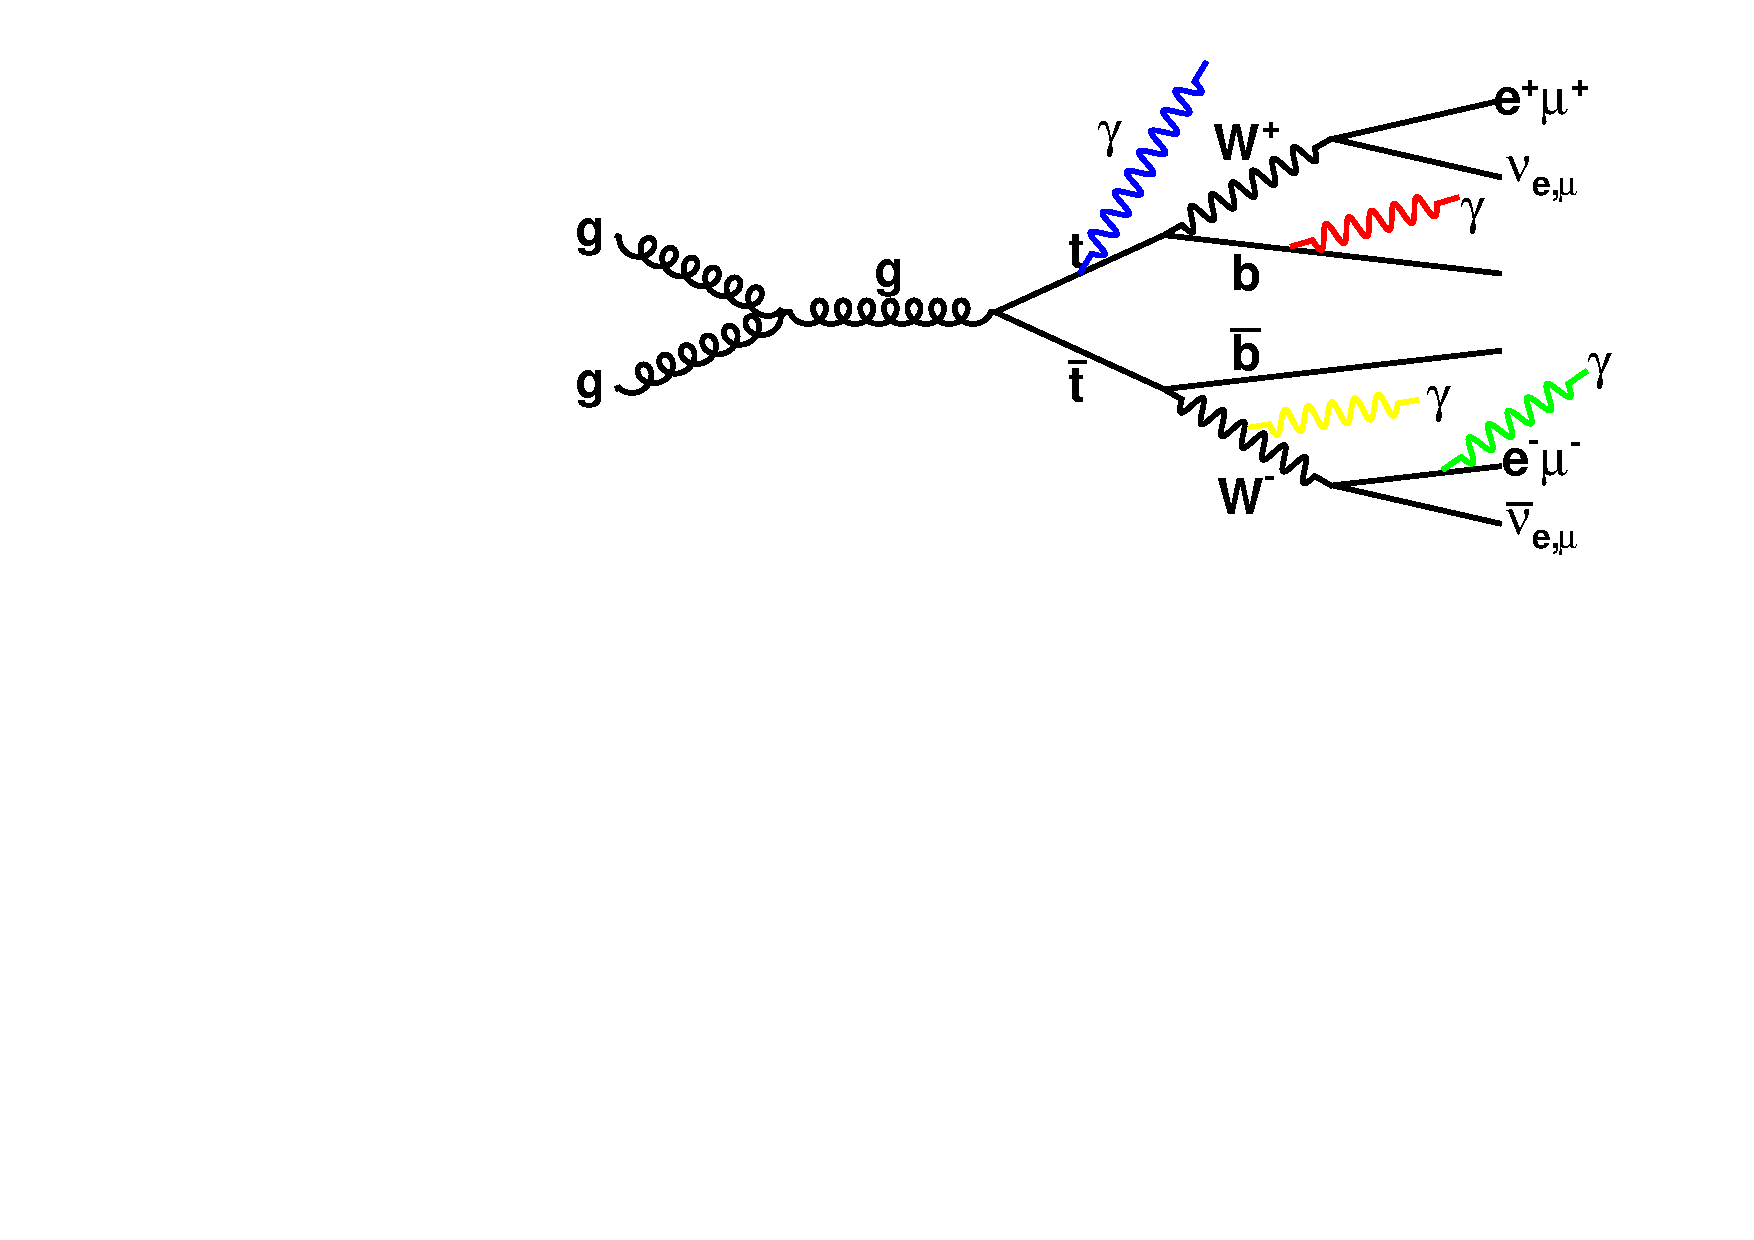
\includegraphics[width=0.9\textwidth]{Figures/ttgammaFeynmanDiagram.pdf}
\end{center}
\caption{Feynman diagram depicting our signal $t\bar{t}+\gamma$ production process in the dilepton channel showing all available decay modes and particles which could possibly radiate a photon.}
\label{fig-ttgammaFeynmanDiagram}
\end{figure}

\subsection{$t\bar{t}+\gamma$ background processes} \label{subsec-ttgammabackgrounds}

\begin{figure} [h!]
\begin{center}
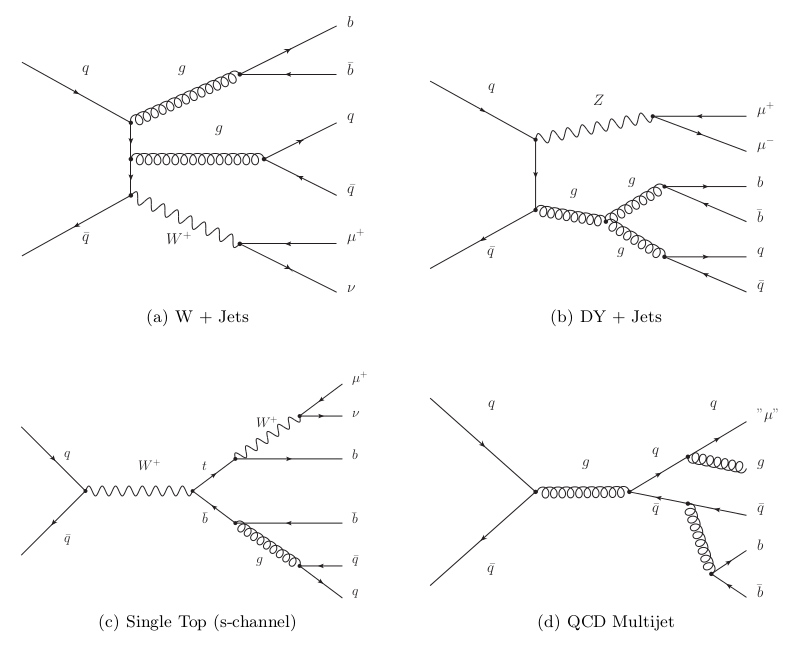
\includegraphics[width=\textwidth]{Figures/BackgroundDiagrams.png}
\end{center}
\caption{Examples of Feynman graphs of the considered $t\bar{t}$ backgrounds. QCD showering is necessary in all cases to obtain the required jet multiplicity \cite{ttgammabackgroundestimation}.}
\label{fig-SignalBackgrounds}
\end{figure}

Many processes produced in collisions at the LHC mimic top quark pair decay, and as a result it is important that we glean a good understanding of these background processes in order to produce an accurate and reliable measurement. The most significant background processes are shown in Figure \ref{fig-SignalBackgrounds}. In order for these signatures to mimic our signal process they must contain at least two oppositely-signed leptons and two jets by $\alpha_S$ showering (gluon radiation). We categorise the background processes for the $t\bar{t}+\gamma$ analysis into top-pair and photon-related backgrounds, and the most significant of these are described in greater detail below.

\begin{description}
	\item[W+Jets] The production of a W boson with additional jet activity is shown in Figure \ref{fig-SignalBackgrounds} (a). In this process a W boson is produced which decays to a single lepton (electron or muon) and corresponding neutrino in the form of missing transverse energy. If there are at least two jets in the final state for this decay, and one jet is wrongly identified as a muon, then it is likely that it would mimic a dileptonic $t\bar{t}$ event. However, leptons and jets originating from the W+Jets process are usually much softer than those of $t\bar{t}$ decay, due to the top quarks large mass. Therefore it is even less probable that jets from W+Jets are b-tagged jets, which are required in our signal process, thus by implementing cuts on the transverse momenta of jets and leptons will reduce the probability of a false signal identification.  
	\item[DY+Jets] The Drell-Yan plus jets process is similar to W+Jets, and is the production of a $Z^0$ boson or photon with additional jets. The bosons then produce two oppositely signed electrons or muons, and with the additional jet activity this results in the same final state as our signal process. Therefore, several techniques must be applied to veto on/reduce this background, such as placing a veto on events that fall into the window such that the invariant mass of the two final state leptons form the Z mass, and also placing a requirement on the missing transverse energy of the event as the DY+Jets process does not include neutrinos. Similar to the W+jets background process, the yield can be drastically reduced by placing a requirement of at least two jets, where one is a b-tagged jet, in the final state. 
	\item[Single Top] We observe single top quark contributions in three channels: s-channel, t-channel, and associated with a W boson (see Figure \ref{fig-singletopProductionLHC}). Although the cross-section is small for these processes, they may contribute significantly to the selection of top pairs, due to their event topology. Their signature may still contain the same final state particles as the dilepton $t\bar{t}$ channel, thus mimicking our signal. Single top production generally contains a lower number of jets in the final state, compared to $t\bar{t}$, however additional jets can emerge from initial and final state radiation (ISR/FSR).  
	\item[QCD Multi-jet] Due to the topology of dilepton events, and the energy of jets originating from QCD being low, we deem this background negligible and do not include it in this analysis. 
	\item[Other $t\bar{t}$ decay modes] Top pair decays other than the dilepton channel (such as the semi-leptonic, fully hadronic, and decay modes that involve tau leptons) are not treated separately. As these decay modes may radiate a photon, it is possible that they can contribute to the $t\bar{t}+\gamma$ signal yield. This is however considered to be small.  
\end{description}

Other background processes, such as diboson production, are considered negligible and are not included due to their very small cross-sections and selection efficiencies.

\subsection{Backgrounds of photon signature}

Photon related background processes are subdivided into three classes. The first two of these comprise the irreducible backgrounds (backgrounds which contain real photons) radiated from initial state partons (ISR), shown in Figure \ref{fig-BackgroundISR}, and photons radiated from final state partons in the hard scattering interactions (FSR), shown in Figure \ref{fig-BackgroundFSR}. The third category contains what we call ``fake photons" originating from electrons passing the same cuts as photons, and jets reconstructed as photons. It is assumed that photon showering in background samples describes the photon background sufficiently for these events. 

%%%%%%%%%%%%%%%

\newpage

\begin{figure} [h!]
\begin{center}
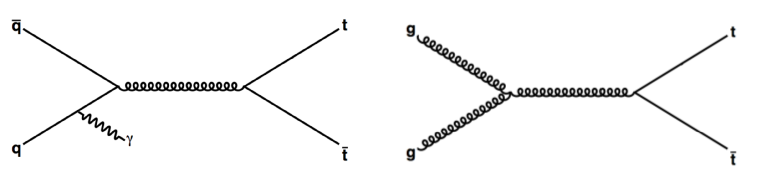
\includegraphics[width=\textwidth]{Figures/BackgroundISR.png}
\end{center}
\caption{Background of photon identification: Initial state radiation (ISR). Left: Quark fusion. Right: Gluon fusion does not give rise to ISR as photons couple to charge (based on \cite{photonbackgrounds}).}
\label{fig-BackgroundISR}
\end{figure}

\begin{figure} [h!]
\begin{center}
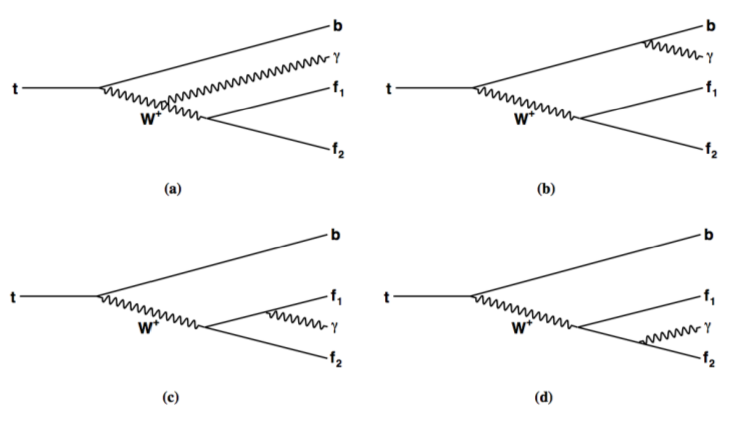
\includegraphics[width=\textwidth]{Figures/BackgroundFSR.png}
\end{center}
\caption{Background of photon identification: Final state radiation (FSR). All charged particles in the top-pair decay tree contribute to FSR \cite{photonbackgrounds}.}
\label{fig-BackgroundFSR}
\end{figure}


\subsection{Top quark anomalous couplings}

The measurement of the couplings between the known fermions and bosons is a standard tool in the search for physics beyond the Standard Model. At the LHC top quarks are produced in copious amounts, allowing us to probe top couplings to a great precision. The large mass of the top quark is directly related to the effects of new physics on its couplings such that deviations from Standard Model predictions may be detectable, therefore the LHC provides the perfect environment in which to study such effects.

The top quark provides a direct test of the quark-photon vertex which is unique among the quarks, thus there is great interest as to the determination of the coupling of the top quark and photon, and probing the $t\bar{t}\gamma$ channel at the LHC with an energy of 8 TeV provides directly explore the top quarks role in the mechanism of electroweak symmetry breaking. Any deviation from that of SM prediction would imply an anomalous structure of the quark-photon vertex, and would thus reveal any physics beyond that of the Standard Model, such as exotic quarks, SUSY, and technicolour, as described in Section \ref{subsec-SMFailures}. 

In order to successfully create a model of interactions between fermions and bosons, we require a good enough parametrisation of the interactions in the form a Lagrangian. We can write a general parametrisation for the on-shell interaction of two fermions ($f_i$, $f_j$) and a boson ($V = W,Z,\gamma,g$) as

\begin{equation}
\begin{split}
\lumi^{OS}_{Vf_if_j} = & \bar{f}_j\gamma^{\mu} (\mathcal{A}_L P_L + \mathcal{A}_R P_R)f_i V_{\mu} \\
& + \bar{f}_j i \sigma^{\mu \nu} q_{\nu}(\mathcal{B}_L P_L + \mathcal{B}_R P_R) f_i V_{\mu} + \text{h.c.}
\end{split}
\end{equation}

where $q = p_i - p_j$ is the momentum of the outgoing boson and $\mathcal{A}_{L,R}$, $\mathcal{B}_{L,R}$ are form factors, which in general may depend on $q^2$, however for the flavour-conserving photon and gluon vertices we have $\mathcal{A}_L = \mathcal{A}_R$ and for flavour-changing $\mathcal{A}_{L,R} = 0$ due to gauge symmetry. 

A set of dimension-six gauge-invariant operators, $O_x$, known as effective operators, can be found to parametrise quark couplings up to a scale $\Lambda$ \cite{anom-coups}. They appear linearly in an interaction Lagrangian, which is written in the form of a Taylor expansion, with complex effective coefficients $C_x$:

\begin{equation} \label{eqn-EffectiveOperators}
\lumi^{eff.} = \sum \frac{C_x}{\Lambda_x}O_x + ... ,
\end{equation}

Among the operators defined in the effective Lagrangian \cite{Buchmuller:1985jz} fourteen contribute to the electroweak anomalous couplings. These are as so:

\begin{align}
& O^{(3, i, j}_{\phi q} = i(\phi^{\dagger}\tau^I D_{\mu} \phi)(\bar{q}_{Li}\gamma^{\mu}\tau^I q_{Lj}), \quad & O^{ij}_{Du} = (\bar{q}_{Li} D_{\mu} u_{Rj}) D^{\mu} \tilde{\phi}, \\
& O^{(1, i, j)}_{\phi q} = i(\phi^{\dagger} D_{\mu} \phi)(\bar{q}_{Li}\gamma^{\mu} q_{Lj}), \quad & O^{ij}_{\bar{D}u} = (D_{\mu} \bar{q}_{Li} u_{Rj}) D^{\mu} \tilde{\phi}, \\
& O^{ij}_{\phi \phi} = i(\phi^{\dagger} D_{\mu} \phi)(\bar{u}_{Ri}\gamma^{\mu} d_{Rj}), \quad & O^{ij}_{Dd} = (\bar{q}_{Li} D_{\mu} d_{Rj}) D^{\mu} \phi, \\
& O^{ij}_{\phi u} = i(\phi^{\dagger} D_{\mu} \phi)(\bar{u}_{Ri}\gamma^{\mu} d_{Rj}), \quad & O^{ij}_{\bar{D}d} = (D_{\mu} \bar{q}_{Li} d_{Rj}) D^{\mu} \phi, \\
& O^{ij}_{uW} = (\bar{q}_{Li} \sigma^{\mu \nu} \tau^I u_{Rj})\tilde{\phi} W^I_{\mu \nu}, \quad & O^{ij}_{qW} = \bar{q}_{Li} \gamma^{\mu} \tau^I D^{\nu} q_Lj W^I_{\mu \nu}\\
& O^{ij}_{dW} = (\bar{q}_{Li} \sigma^{\mu \nu} \tau^I d_{Rj})\phi W^I_{\mu \nu}, \quad & O^{ij}_{qB} = \bar{q}_{Li} \gamma^{\mu} D^{\nu} q_Lj B_{\mu \nu}\\
& O^{ij}_{uB\phi} = (\bar{q}_{Li} \sigma^{\mu \nu} u_{Rj})\tilde{\phi} B_{\mu \nu}, \quad & O^{ij}_{uB} = \bar{u}_{Ri} \gamma^{\mu} D^{\nu} u_Rj B_{\mu \nu}
\end{align} \label{eqn-effectiveOperators}

for different flavours represented by the indices $i,j = 1,2,3$. $\bar{q}_{Li}$, $u_{Ri}$, and $d_{Ri}$ represent the quark fields as shown in Section \ref{subsec-ElectroweakTheory}. The operators where we have $i = j = 3$ contribute to the electroweak coupling processes $Wtb$, $Zt\bar{t}$, and $\gamma t\bar{t}$. 

% \cite{Whisnant:1997qu} \cite{Yang:1997iv}

%%%%%%%%%%%%%%%%%%%%%%%%%%%%%%%%%%%%%%%%%

\subsection{The top-photon vertex}

\begin{figure} 
\begin{center}
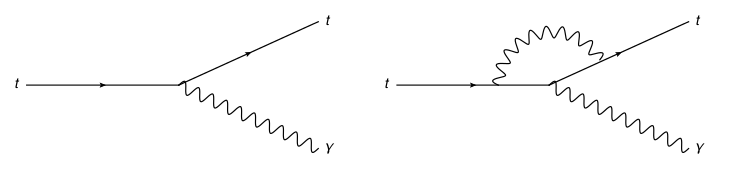
\includegraphics[width=\textwidth]{Figures/TopPhotonVertex.png}
\end{center}
\caption{Top-photon vertex. Left: Leading Order (LO). Right: One-Loop correction (NLO).}
\label{fig-TopPhotonVertex}
\end{figure}

The general expression for the interaction Lagrangian for the top-photon ($\gamma t \bar{t}$) vertex (shown in Figure \ref{fig-TopPhotonVertex}) can be parametrised in terms of the dimension-six operators and written, not including the redundant operators, in the form \cite{anom-coups}:

\begin{equation} \label{eqn-interactionlagrangian}
\lumi_{\gamma t\bar{t}} = -eQ_t\bar{t}\gamma^{\mu}tA_{\mu} - e\bar{t}\frac{i\sigma^{\mu\nu}q_{\nu}}{m_t}(d^{\gamma}_V+id^{\gamma}_A\gamma^5)tA_{\mu}
\end{equation}

The first term in Equation \ref{eqn-interactionlagrangian} is a purely SM contribution, and is linear with respect to electrical charge of the top, $Q_t$, such that the bare $t\bar{t}+\gamma$ cross-section is proportional to the square of the top-quark charge. The second term is described by the vector and axial form factors, $d^{\gamma}_V$ and $d^{\gamma}_A$, which arise from the contributions of first-order loop corrections, representing the magnetic and electric dipole moment of the top quark (where the latter is CP-violating), respectively. The couplings, $d^{\gamma}_V$ and $d^{\gamma}_A$, are real and comprise the operators $O^{33}_{uB\phi}$ and $O^{33}_{uW}$ from the eight effective operators described previously mentioned. They parametrise deviations from SM expectations of the form factors, $d^{\gamma}_V$ and $d^{\gamma}_A$, as such:

\begin{align}\label{eqn-smparameterisations}
\delta d^{\gamma}_V = \frac{\sqrt{2}}{e}\text{Re}[c_W C^{33}_{uB\phi} + s_W C^{33}_{uW}]\frac{vm_t}{\Lambda^2} \\
\delta d^{\gamma}_A = \frac{\sqrt{2}}{e}\text{Im}[c_W C^{33}_{uB\phi} + s_W C^{33}_{uW}]\frac{vm_t}{\Lambda^2}
\end{align}

where $\delta d^{\gamma}_V$ and $\delta d^{\gamma}_A$ only receive non-zero contributions from phenomena beyond the SM. We are able to obtain a measurement of these constants by analysing the magnetic and electric dipole moments of the top quark. We note that the $\gamma^{\mu}$ term does not receive corrections from the dimension-six operators. If we had included the redundant effective operators ($O_{Wq}$, $O_{Bq}$, $O_{Bu}$) then the first two would incorporate additional corrections of $\sim q^2 \bar{t}_L \gamma^{\mu} t_R A_{\mu}$ and the last $q^2 \bar{t}_R \gamma^{\mu} t_R A_{\mu}$, no-vanishing only when the photon is off-shell.

The magnetic dipole moment of the top quark is studied by measurements of spin correlation, whereas the electric dipole moment can be investigated through the $t\gamma$ vertex. Deviations from SM contributions are expected to manifest in the photon energy spectrum and angular photon distributions.

Measuring $t\bar{t}+\gamma$ provides a direct test of the electromagnetic coupling of the top quark in a way that is complementary to analyses that include an ``exotic" top quark with a charge of -4/3e \cite{top-charge}. A sketch of the potential photon E$_T$ in relation to having extra couplings, or having a charge of $-4/3e$ can be seen in Figure \ref{fig-TopChargeSketch}. One issue when investigating the $t\bar{t}+\gamma$ process is the large irreducible background of photons that are radiated by charged particles other than the top quark. It has also been proved that the interference of photon production from initial state radiation (ISR) and final state radiation (FSR) can not be deemed negligible \cite{topchargemeasurement}. This is also discussed with respect to Monte Carlo signal generation in Section \ref{sec-mcsim}. Thus only inclusive observables of $t\bar{t}+\gamma$ can be probed, as we are unable to trace the photon back to its parent particle. We will also treat on- and off-shell radiation collectively. We will discuss prompt photon backgrounds in Section \ref{chap-EventSelection}. 

\begin{figure} 
\begin{center}
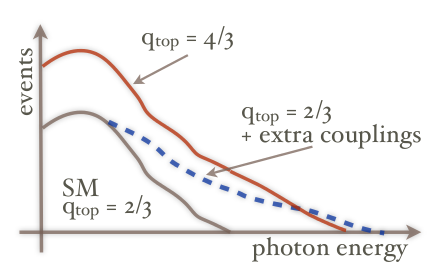
\includegraphics[width=0.6\textwidth]{Figures/TopChargeHeiner.png}
\end{center}
\caption{Sketch of expected photon energy spectra. The reference line is Standard Model ($q_{top} = +2/3$). A deviation of the top electrical charge yields a differently normalized photon rate ($q_{top} = −4/3$). Extra couplings, e.g. a large electrical dipole moment manifests in different kinematic shapes (dashed line). \cite{heinerthesis}}
\label{fig-TopChargeSketch}
\end{figure}

\subsection{Previous measurements}

Presently, the determination of the operators $C^{33}_{uB\phi}$ and $C^{33}_{uW}$ is not possible due to the statistical significance of recorded events at the LHC being low. This will become more accessible at higher centre-of-mass energy and luminosity. Until then, benchmark studies have been undertaken \cite{photonbackgrounds}.

The CDF experiment at the Tevatron, along with the CMS and ATLAS experiments at the LHC, have measured the inclusive $t\bar{t}+\gamma$ production cross-section at $\sigma^{CDF}_{t\bar{t}+\gamma} = 0.18 \pm 0.08$ pb \cite{CDFttgamma}, $\sigma^{CMS}_{t\bar{t}+\gamma} = 2.4 \pm 0.2 (\text{stat}) \pm 0.6 (\text{syst.})$ \cite{CMS-PAS-TOP-13-011}, and $\sigma^{ATLAS}_{t\bar{t}+\gamma} = 2.0 \pm 0.5 (\text{stat}) \pm 0.7 (\text{syst.}) \pm 0.08 (\text{lumi})$ pb at 7 TeV \cite{ATLASttgamma}, respectively. The SM expectations for these values are given as $\sigma^{Tevatron}_{t\bar{t}+\gamma} = 0.17 \pm 0.003$ pb and $\sigma^{LHC}_{t\bar{t}+\gamma} = 2.1 \pm 0.4$ pb, respectively, and thus the measurements observed are in accordance to those theorised. 

In relation to the electrical charge of the top quark, the CMS and ATLAS experiments have also performed analyses, hypothesis tests, where the final state charges of the top quark are combined, and both yield similar results. The experiments concluded that an electrical charge of $Q_t = -4/3e$ could be excluded  with a high significance \cite{topchargeconstraints, ATLAStopcharge}.

Other top quark couplings have been measured at the Tevatron and the LHC. The structure of the $Wtb$ vertex has been investigated in 
helicity measurements of top quark correlated W bosons at the Tevatron and LHC, putting limits on anomalous couplings \cite{CDFD0combination, 
Whelicitytoppair, Wpolarisation}. The strength of $tW$ couplings can be tested through single top quark production and has been found to be 
consistent with SM expectations \cite{tsinglet, singlet}. Also, the inclusive $t\bar{t}W$ and $t\bar{t}Z$ production cross-sections have been 
measured by CMS to be $\sigma_{t\bar{t}W} = 170^{+90}_{-80}(\text{stat}.) \pm 70(\text{syst}.)$ fb and $\sigma_{t\bar{t}Z} = 200^{+80}_{-70}(\text{stat}.) ^{+40}_{-30}(\text{syst}.)$ fb, respectively, with the combined $t\bar{t}V$ cross-section as $\sigma_{t\bar{t}V} = 380^{+100}_{-90}
(\text{stat}.)^{+80}_{-70}(syst.) $ fb, and exclusion limits on anomalous couplings are set \cite{Khachatryan:1712680}. Another focus in the 
area is flavour changing neutral currents (FCNC) in top decays, $t \to qZ$ and $t \to q\gamma$ are also currently being studied. Limits are set 
for these processes \cite{tqZ, FCNC}, which confirm SM FCNC suppression. 

It is important to note that a measurements of $t\bar{t}+\gamma$ are extremely challenging at the LHC with the current centre-of-mass energy 
and luminosity. This is due to the limited four-momentum resolution of partons, pile-up, and large background from QCD multi-jet events. It has 
been estimated that a 10\% resolution of the top quark's charge will be available at $\sqrt{s} = 14$ TeV with 10 fb$^{-1}$ \cite{
topchargemeasurement}. As the energy is increased at the LHC the gluon fusion process becomes more dominant and thus fewer photons can be 
emitted in the form of initial state radiation. A high energy $e^+e^-$ collider would be preferable for this study as it would be a much 
cleaner working environment, such that we could obtain a 5--10\% precision on axial form factor $d^{\gamma}_A$ can be achieved with 10 fb$^{-1}$
at $\sqrt{s} = 500$ GeV \cite{linearcollider}.
